\documentclass[14pt]{extarticle}
\usepackage{amsmath}
\usepackage{amssymb}
\usepackage{tikz}
\usetikzlibrary{calc}
%\usetikzlibrary{trees}
\usepackage{hyperref}
\usepackage{graphicx}
\graphicspath{ {../../chap07/} }
\usepackage[top=0.75in, bottom=0.75in, left=0.75in, right=0.75in]{geometry}
\newcommand*{\Scale}[2][4]{\scalebox{#1}{\ensuremath{#2}}}%
\usepackage[shortlabels]{enumitem}
\usepackage[most]{tcolorbox}
\definecolor{bg}{RGB}{255,249,227}
% \usepackage{showframe}
\title{\vspace{-5ex}Math 208 Section 7.2}
\date{\vspace{-10ex}}
\usepackage{multicol}
\setlength{\columnsep}{1cm}


\begin{document}
\maketitle		
\section*{Homework, Reading, and Other}
\begin{itemize}
	\item Section 5.2
	\item Section 5.3
	\item Section 7.2
\end{itemize}

\section*{Quiz}

\section*{Goals}
\begin{itemize}
	\item Understand basic concepts of a set
	\item Use set notations
	\item State meaning of Union, Intersection, Disjoint, and Complement
	\item Analyze Venn diagrams and sets
\end{itemize}

\section*{7.2 Sets}
A set is any collection of objects. We denote a set using Capital letters and each object of a set is called a \textit{member} or \textit{element}.

\subsection{Notation}
\begin{itemize}
	\item $x \in A$ means x is an element of A.
	\item $x \notin A$ means x is not an element of A.
	\item $\emptyset$ is an empty set or a set with no members. Note that $\emptyset \neq \{\emptyset\}$.
	\item $S = \{1,x,car,8,z\}$ means S is a set containing a variety of elements.
	\item The order of elements in a set does not matter.
	\item $A \subset B$ means every element of A is also an element of B. Say this as "A is a subset of B". 
	\item $A \not\subset B$ means not every element of A is also an element of B. Say this as "A is not a subset of B".
	\item $S = P$ means S and P have exactly the same elements. Note that if $S \subset P$ and $P \subset S$, then $S = P$.
\end{itemize}
	

\subsubsection{Examples}
Given:
\begin{align*}
	A = \{-3,-1,1,3\} & & B=\{-1,1,-3,3\} & & C  \{–3, –2, –1, 0, 1, 2, 3\}
\end{align*}
Then
\begin{align*}
	A &= B & A &\subset C & A &\subset B \\
	C &\neq A & C &\not\subset A & B &\subset A \\
	B &\neq \emptyset & 2 &\notin A & 2 &\in C
\end{align*}

\subsection{Venn Diagrams}
An easy way to visualize set, their membership, and their interactions is using a Venn diagram.
\begin{center}
	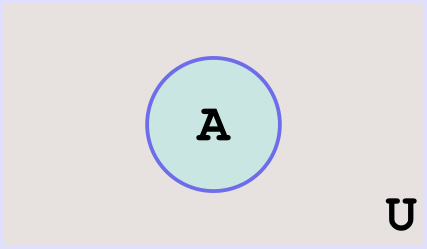
\includegraphics[width=0.5\linewidth]{venn-1}
\end{center}
In this Venn diagram, U is all of the space and A is the space indicated by the circle. A may represent any set we choose.

\begin{tcolorbox}[enhanced jigsaw,colback=bg,boxrule=0pt,arc=0pt] 
	\begin{enumerate}
		\item \textbf{Union}: $A \cap B$ all items that are elements of A or B.
		\item \textbf{Intersection}: $A \cup B$ all items that are elements of both A and B.
		\item \textbf{Complement}: $A'$ all items that are not elements of A.
		\item \textbf{Disjoint}: $A$ and $B$ are disjoint when their intersection is empty, i.e., $A \cap B = \emptyset$.
	\end{enumerate}
\end{tcolorbox}

Using the below Venn diagram, we have that:
\begin{align*}
	A &= \{1,2,5,6\} &  B&= \{3,4,5,6\}  & C &= \{8\}\\
	A \cup B &= \{1,2,3,4,5,6\} & A \cap B&= \{5,6\} & A \cap C &= \emptyset\\
	A' &= \{3,4,5,6,7,8\} & (A\cup B)' &= \{7,8\} & & \\
	&\text{C is disjoint with both A and B}
\end{align*}
\begin{center}
	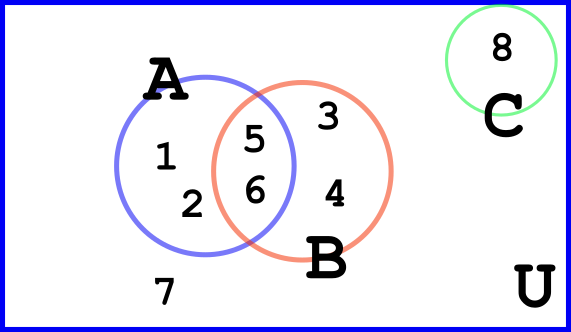
\includegraphics[width=0.5\linewidth]{venn-2}
\end{center}
Often, we are interested in how many elements are in a set. This is indicated by $n(A)$. For the above Venn diagram, we have:
\begin{align*}
	n(A) &= 4  & n(B)&= 4  & n(C) &= 1 \\
	n(A \cup B) &= 6 & n(A \cap B)&= 2 & A \cap C &= 0 \\
	n(A') &= 4 & n(A\cup B)' &= 2 & & \\
\end{align*}

\noindent\rule{\textwidth}{1pt}
{\footnotesize Copyright (C) 2021 Garold Dalton --- Released under GNU General Public License v3.0}


\cleardoublepage


\end{document}
